\documentclass[xcolor={dvipsnames},aspectratio=169]{beamer}
\usepackage[utf8]{inputenc}
\usepackage{hyperref}
\usepackage{xurl}
\usepackage{microtype}
\usetheme{Madrid}
\usecolortheme{default}
\setbeamertemplate{enumerate items}[default]
\setbeamercolor*{structure}{bg=white,fg=black}

\definecolor{MQRed}{RGB}{166,25,46}       % Red
\definecolor{MQDeepRed}{RGB}{118,35,47}   % Deep Red
\definecolor{MQBrightRed}{RGB}{214,0,28}  % Bright Red
\definecolor{MQMagenta}{RGB}{198,0,126}   % Magenta
\definecolor{MQPurple}{RGB}{128,34,95}    % Purple
\definecolor{MQCharcoal}{RGB}{55,58,54}   % Charcoal
\definecolor{MQSand}{RGB}{214,210,196}    % Sand

\setbeamercolor{normal text}{fg=MQCharcoal}
\setbeamercolor{structure}{fg=MQDeepRed}
\setbeamercolor{title}{fg=MQRed, bg=MQSand}
\setbeamercolor{section in toc}{fg=MQRed}
\setbeamercolor{subsection in head/foot}{bg=MQDeepRed,fg=white}

\usepackage{times,url}

\setbeamertemplate{footline}{BERTopic summarisation of
student responses to an in-class survey --- CC-BY Ballsun-Stanton and Hurley}



%------------------------------------------------------------
%This block of code defines the information to appear in the
%Title page
\title[Berttopic] %optional
{BERTopic summarisation of
student responses to an in-class survey}

\subtitle{Assessing the use of Bing Chat in PICT2020's assessments}

\author[Brian Ballsun-Stanton] % (optional)
{Brian Ballsun-Stanton (FoA) and Vincent Hurley (FoA, SSC)}


\date[13 December 2023] % (optional)
{Sociolinguistics through Corpus Research, December 2023}


%End of title page configuration block
%------------------------------------------------------------


\begin{document}

%The next statement creates the title page.
\frame{\titlepage}


%---------------------------------------------------------
%This block of code is for the table of contents after
%the title page
\begin{frame}
\frametitle{Table of Contents}
\tableofcontents
\end{frame}
%---------------------------------------------------------


\section{Generative AI in PICT2020 Assessments}

%---------------------------------------------------------
%Changing visivility of the text
\begin{frame}{Generative AI in FoA undergraduate teaching in 2023}

\begin{itemize}
    \item Faculty of Arts experiment in Generative AI 
    \begin{itemize}
        \item PICT2020 --- Policing and Crime
        \item GRMN1020 --- German 2
    \end{itemize}
    \item AI ``Enabled'' and AI ``Agnostic''
\end{itemize}

\end{frame}

\begin{frame}
\frametitle{PICT2020 --- Policing and Crime}

\begin{itemize}
    \item Authentic assessment: Goal of the unit is to deliver a 5 minute oral review brief
    \item Assessments:
    \begin{itemize}
        \item Media review (Interrogate with and without Bing Chat)
        \item Annotated Bibliography
        \item Peer review practice + AI feedback
        \item 5 minute oral review
        
    \end{itemize}
    \item AI ``Enabled'' and AI ``Agnostic'' assessment.
    \item Faculty's experiment in what happens when students are taught how to use and think about LLMs and then expected to apply that in every assessment.
\end{itemize}

\end{frame}


\begin{frame}{Problem: how did students feel about generative AI in their assessments?}

\begin{itemize}
    \item Was the training in using Bing Chat sufficient?
    \item Did they feel the unit was more authentic?
    \item Did they appreciate working with Large Language Models?
    \item Did it enhance the learning experience?
\end{itemize}

\end{frame}

\begin{frame}
\frametitle{Data: required and graded end of unit survey}

\begin{itemize}
    \item n=175
    \item 2 Likert
    \item 2 Boolean
    \item 11 Qualitative
\end{itemize}

\end{frame}

\section{Analysis}

\begin{frame}
\frametitle{Analysis in a hurry}

\begin{itemize}
    \item n=175
    \item 2 Likert
    \item 2 Boolean
    \item 11 Qualitative
\end{itemize}

Two academics sitting in front of ChatGPT 4.

\end{frame}


\begin{frame}{Analysis in a hurry}

Charting quant data, LDA for qual data, all within a single GPT-4 chat.

\begin{columns}
\begin{column}{0.3\textwidth}
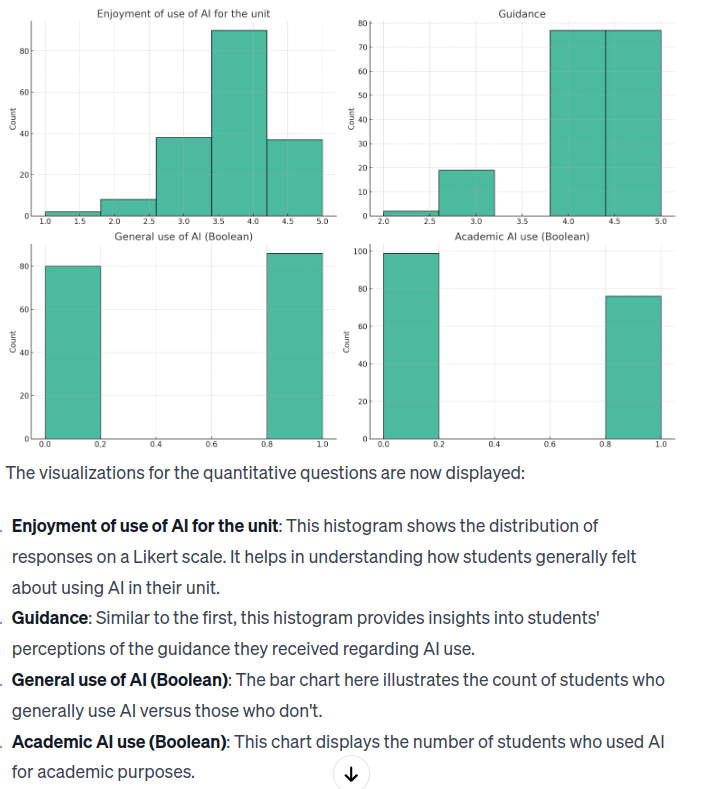
\includegraphics[width=\textwidth]{Screenshot from 2023-12-12 11-28-52.png}
\end{column}
\begin{column}{0.3\textwidth}
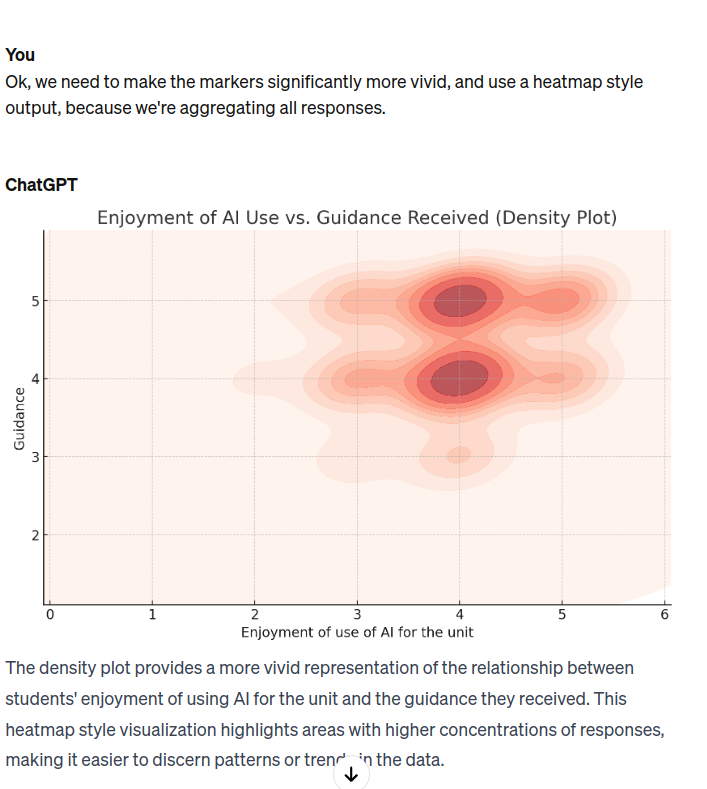
\includegraphics[width=\textwidth]{Screenshot from 2023-12-12 11-30-43.png}
\end{column}
\begin{column}{0.3\textwidth}
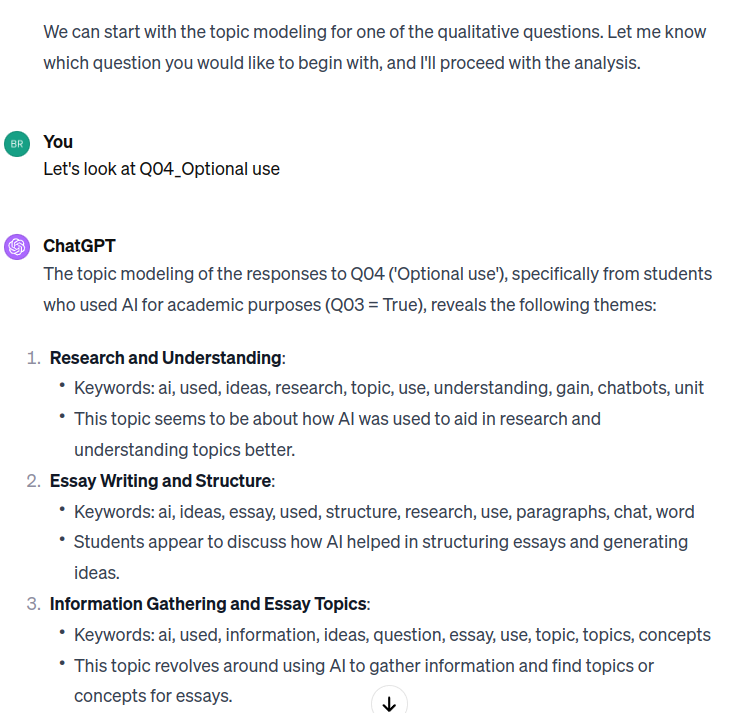
\includegraphics[width=\textwidth]{Screenshot from 2023-12-12 11-31-54.png}
\end{column}
\end{columns}

{\tiny
\url{https://chat.openai.com/share/9ba21815-3537-4bf4-b0e4-1b4c8d7b62a1}
}

\end{frame}

\begin{frame}{BERTopic}
\begin{columns}
\begin{column}{0.5\textwidth}
    \begin{itemize}
    \item LDA topic modelling is awfully close to random noise. 
    \item Very dependent on initial conditions and amounts of buckets.
    \item BERTopic uses the Sentence Transformer BERT to do embeddings and sentence clustering using Large Language Models. (https://maartengr.github.io/BERTopic)
\end{itemize}
\end{column}
\begin{column}{0.5\textwidth}
    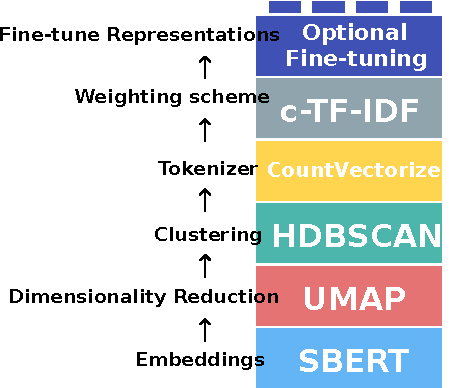
\includegraphics[width=\textwidth]{bert.pdf}
    {\tiny \url{maartengr.github.io/BERTopic/algorithm/algorithm.html}}
\end{column}
\end{columns}

    
\end{frame}

\begin{frame}{Analysis in a Day}
\begin{itemize}
    \item Use ChatGPT 4 to make the Python harness for the analysis:
\end{itemize}
\begin{quote}
    Hi ChatGPT. Today we're going to be preparing a code harness to do some analysis with python using VSCode and Github Copilot. However, we're going to develop the function stubs, classes, docstrings, and stubbed doctests here in preparation. I would like you to take the role of a software architect when designing these things. Ask for clarification where needed.

We will be working through text summarisation of a survey, using BERTopic topic modelling (search the web for details) to extract topics per question, returning texts per question with that topic, and then using this chat interface to summarise those texts. The output of this program should be a series of text files, plus BERTopic visualisations. Each text file should have a prompt, the topic or topics grouped together by BERTopic, and the texts for summarisation. ...
\end{quote}
{\tiny \url{https://chat.openai.com/share/3c12945a-7c14-4f2a-8626-ca4a5fce5488}}    
\end{frame}
\section{BERTopic}
\begin{frame}{Writing code}


\begin{columns}

\column{0.45\textwidth}
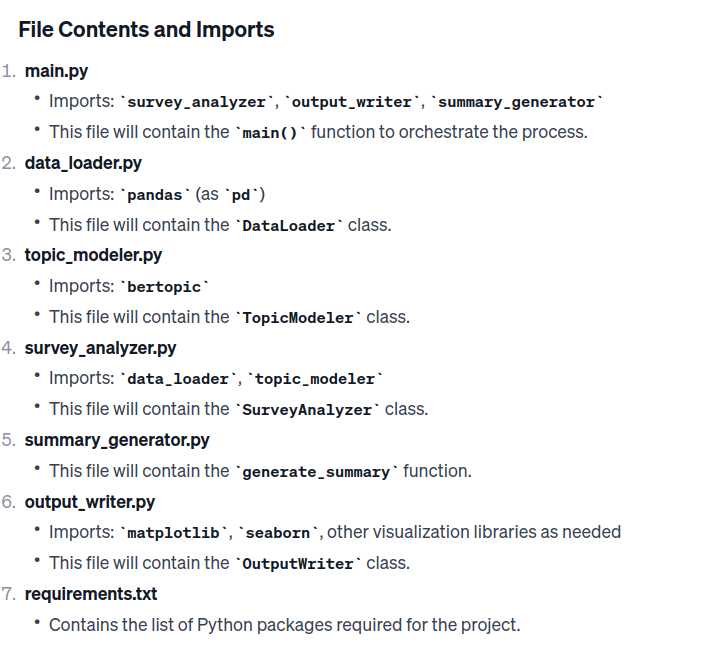
\includegraphics[width=\textwidth]{Screenshot from 2023-12-12 11-42-45.png}
\column{0.05\textwidth}
$\rightarrow$
\column{0.45\textwidth}
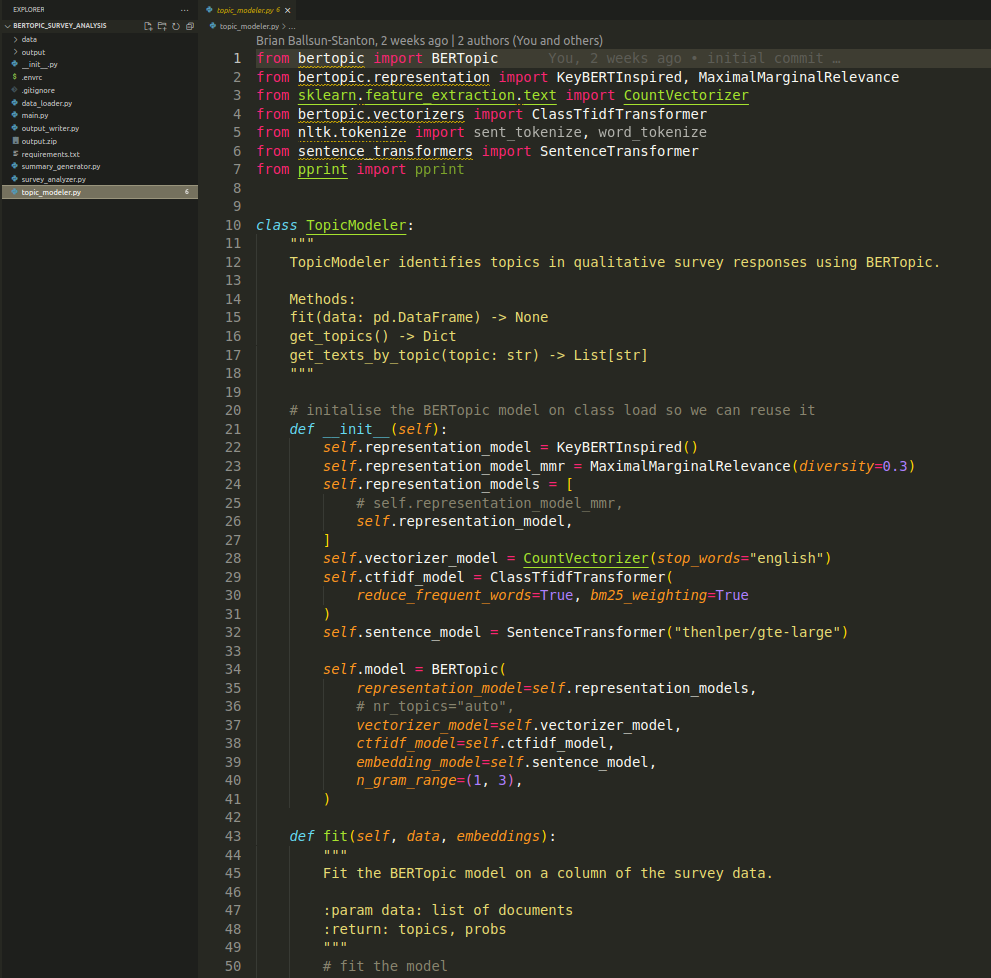
\includegraphics[width=\textwidth]{Screenshot from 2023-12-12 11-46-10.png}
\end{columns}
Through the magic of Github Copilot and a decent GPU. 
\end{frame}
%---------------------------------------------------------
\begin{frame}{Per question topic modelling, with representative output}
    Output is a per question document topic model, plus representative text files.

    \begin{columns}

\column{0.5\textwidth}
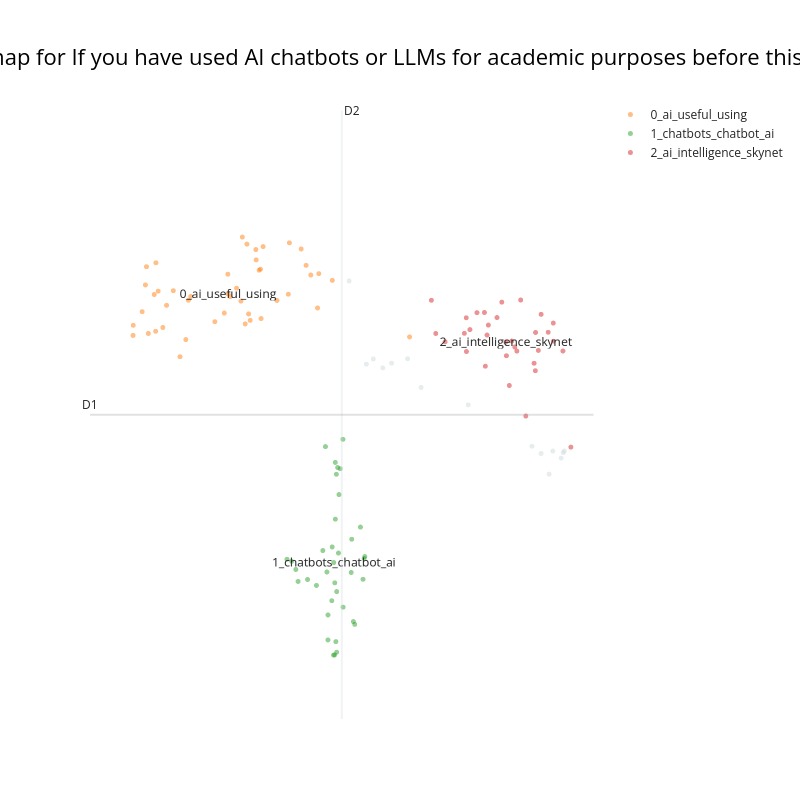
\includegraphics[width=\textwidth]{newplot (1).png}
\column{0.5\textwidth}
\tiny
\begin{verbatim}

Topic: 0, ai, useful, using (1)

Topic Words: 
* chatbots (0.915)
* chatbot (0.914)
* ai (0.888)
* chatgpt (0.855)
* chat (0.847)
* help (0.833)
* learning (0.831)
* using (0.830)
* use (0.827)
* helpful (0.826)


Representative Texts:

* I've used AI chatbots in both my Law and Security Study Degrees. I
  found AI is extremely helpful in gaining ideas for points to research
  on a particular topic.  ...

* The first time I used a form of AI chatbot was Chat GPT for an
  Introduction to computer programming class I did last semester.
  Essentially I used it as a tool to explain to me how certain code was
  used and it's purpose if I didn't have immediate access to assistance
  from my tutor etc. ...

* I have used AI chatbots for academic purposes before this unit,
  specifically ChatGPT. I had not used any other chatbot such as The New
  Bing before this unit. Primarily, I would type in the essay question
  and get an example of an essay for my topic. That way I had a good
  idea how I should structure my assignment and potential topics I could
  cover. This helped me see any blind spots that I had before starting
  my essay. ... 
\end{verbatim}
\end{columns}
\end{frame}

\section{Conclusions}
\begin{frame}{Conclusions}
\begin{itemize}
\item The use of large language models required active teaching
\begin{itemize}
    \item To demonstrate appropriate use
    \item To show correct prompting modes
    \item To model critical reading
\end{itemize}
\item The students were more engaged with authentic assessments, are better prepared to engage with these tools in the future, and were able to cover more content. 
\item The increased efficiency allowed an concomitant increase in complexity, going up Bloom's Taxonomy to Analyse/Evaluate (\url{https://cft.vanderbilt.edu/guides-sub-pages/blooms-taxonomy/}). 
\item This experiment was successful, and it is the job of the Humanities to teach appropriate and effective use of Large Language Models. (But we \textit{must} teach it -- as the students are terrified and \textit{not} digital natives.
\end{itemize}
\end{frame}

% %---------------------------------------------------------
% %Example of the \pause command
% \begin{frame}
% In this slide \pause

% the text will be partially visible \pause

% And finally everything will be there
% \end{frame}
% %---------------------------------------------------------

% \section{Second section}

% %---------------------------------------------------------
% %Highlighting text
% \begin{frame}
% \frametitle{Sample frame title}

% In this slide, some important text will be
% \alert{highlighted} because it's important.
% Please, don't abuse it.

% \begin{block}{Remark}
% Sample text
% \end{block}

% \begin{alertblock}{Important theorem}
% Sample text in red box
% \end{alertblock}

% \begin{examples}
% Sample text in green box. The title of the block is ``Examples".
% \end{examples}
% \end{frame}
% %---------------------------------------------------------


% %---------------------------------------------------------
% %Two columns
% \begin{frame}
% \frametitle{Two-column slide}

% \begin{columns}

% \column{0.5\textwidth}
% This is a text in first column.
% $$E=mc^2$$
% \begin{itemize}
% \item First item
% \item Second item
% \end{itemize}

% \column{0.5\textwidth}
% This text will be in the second column
% and on a second tought this is a nice looking
% layout in some cases.
% \end{columns}
% \end{frame}
% %---------------------------------------------------------


\end{document}